\documentclass{beamer}

\setlength{\leftmargini}{1em}
\setbeamertemplate{itemize item}[circle]
\setbeamertemplate{frametitle}
{
\raggedright\insertframetitle%
}

\usepackage{lipsum}

\usepackage{agda}
\usepackage{apacite}
\usepackage{catchfilebetweentags}
\usepackage{changepage}
\usepackage{babel}
\usepackage{bookmark}

\usepackage{graphicx}

\usepackage[autostyle=true,french=guillemets,maxlevel=3]{csquotes}

\graphicspath{ {images/} }

\usepackage{newunicodechar}
\newunicodechar{∋}{$\ni$}
% \newunicodechar{·}{$\cdot$}
\newunicodechar{⊢}{$\vdash$}
\newunicodechar{⋆}{${}^\star$}
\newunicodechar{Π}{$\Pi$}
\newunicodechar{⇒}{$\Rightarrow$}
\newunicodechar{ƛ}{$\lambdabar$}
\newunicodechar{∅}{$\emptyset$}
\newunicodechar{∀}{$\forall$}
\newunicodechar{ϕ}{$\Phi$}
\newunicodechar{ψ}{$\Psi$}
\newunicodechar{ρ}{$\rho$}
\newunicodechar{α}{$\alpha$}
\newunicodechar{β}{$\beta$}
\newunicodechar{μ}{$\mu$}
\newunicodechar{σ}{$\sigma$}
\newunicodechar{≡}{$\equiv$}
\newunicodechar{Γ}{$\Gamma$}
\newunicodechar{∥}{$\parallel$}
\newunicodechar{Λ}{$\Lambda$}
\newunicodechar{₀}{$~_0$}
\newunicodechar{₁}{$~_1$}
\newunicodechar{₂}{$~_2$}
\newunicodechar{₃}{$~_3$}
\newunicodechar{θ}{$\theta$}
\newunicodechar{Θ}{$\Theta$}
\newunicodechar{∘}{$\circ$}
\newunicodechar{Δ}{$\Delta$}
\newunicodechar{λ}{$\lambda$}
\newunicodechar{⊧}{$\models$}
\newunicodechar{⊎}{$\uplus$}
\newunicodechar{η}{$\eta$}
\newunicodechar{⊥}{$\bot$}
\newunicodechar{Σ}{$\Sigma$}
\newunicodechar{ξ}{$\xi$}
\newunicodechar{ℕ}{$\mathbb{N}$}
\newunicodechar{ᶜ}{${}^c$}
\newunicodechar{Φ}{$\Phi$}
\newunicodechar{Ψ}{$\Psi$}
\newunicodechar{⊤}{$\top$}
\newunicodechar{≐}{$\doteq$}
\newunicodechar{≣}{$\triangleq$}
\newunicodechar{≃}{$\simeq$}
\newunicodechar{≅}{$\cong$}
\newunicodechar{∙}{$\bullet$}
\newunicodechar{ℓ}{$\ell$}
\newunicodechar{ℚ}{$\Q$}
\newunicodechar{ℤ}{$\Z$}
\newunicodechar{⦃}{$\{$}
\newunicodechar{⦄}{$\}$}
\newunicodechar{≤}{$\leqslant$}
\newunicodechar{≥}{$\geqslant$}
\newunicodechar{≟}{$\doteq$}
\newunicodechar{∈}{$\in$}
% \newunicodechar{}{$$}


\newunicodechar{∣}{\ensuremath{\mathnormal{\|}}}
\newunicodechar{∷}{\ensuremath{::}}

\newcommand{\agda}[2]{\ExecuteMetaData[latex/#1.tex]{#2}}

\usetheme{Frankfurt}

\DeclareQuoteStyle{english}
  {\em}
    {\em}
    {\textquotedblleft\em}
    {\em\textquotedblright}

% Information to be included in the title page:
\title{Formalizing Bitcoin prototype \\
  using dependent types in Agda }
\author[Guilherme H. A. Silva]{Guilherme Horta Alvares da Silva}
% \institute{Fundação Getulio Vargas}
\date{2021}


\begin{document}

\frame{\titlepage}

\section{Introduction}

\begin{frame}
\frametitle{Goal}
\begin{itemize}
  \item Using Agda's dependent types to create a formal definition of a crypto currency similar to Bitcoin.
    
\includegraphics[width=8cm, height=5cm]{TwoBitcoins}
\end{itemize}
\end{frame}

\begin{frame}
   \frametitle{Definition}
\begin{itemize}
     \item A cryptocurrency is a decentralized mean of exchange that uses
       blockchain and cryptography to create new currency units and ensure the validity of transactions.
     \item Bitcoin is considered the world's first decentralized digital currency,
       constituting an alternative economic system (peer-to-peer electronic cash system).
       % \cite{nakamoto2008bitcoin}
     \item In this project, I will define cryptographic functions, transactions, block and blockchain.
     \item Distributed system aspects are outside of the scope of this work.
     \end{itemize}
\end{frame}

\begin{frame}
   \frametitle{Ethical Aspects}
\begin{itemize}
  \item In Satoshi Nakamoto's vision, Bitcoin would be minerated by everyone.
    But until today, there are just a few miners in places on Earth.
  \item Mining spends a lot of energy because of the proof of work of Bitcoin.
    However, most of the energy to mine is green. It is usually geothermic energy that would not be used where it was produced.
  \item Other cryptocurrencies, such as Cardano, use Proof of Stake to solve this problem. In addition, mining rewards go to people who have a Proof of Stake cryptocurrency.
\end{itemize}
\end{frame}

\begin{frame}
  \frametitle{Imports}
\begin{code}

module main where

open import Data.Nat
open import Data.List
open import Data.Unit hiding (_≤_; _≟_)
open import Data.Empty
open import Data.Sum hiding (map)
open import Data.Fin hiding (_+_; _≥_; _≤_; _-_; _≟_)
open import Data.Product hiding (map)
open import Function
open import Relation.Binary.PropositionalEquality
open import Relation.Nullary
open import Utils

\end{code}
\end{frame}

\section{Crypto Functions}

\begin{frame}
  \frametitle{Bitcoin Account}
    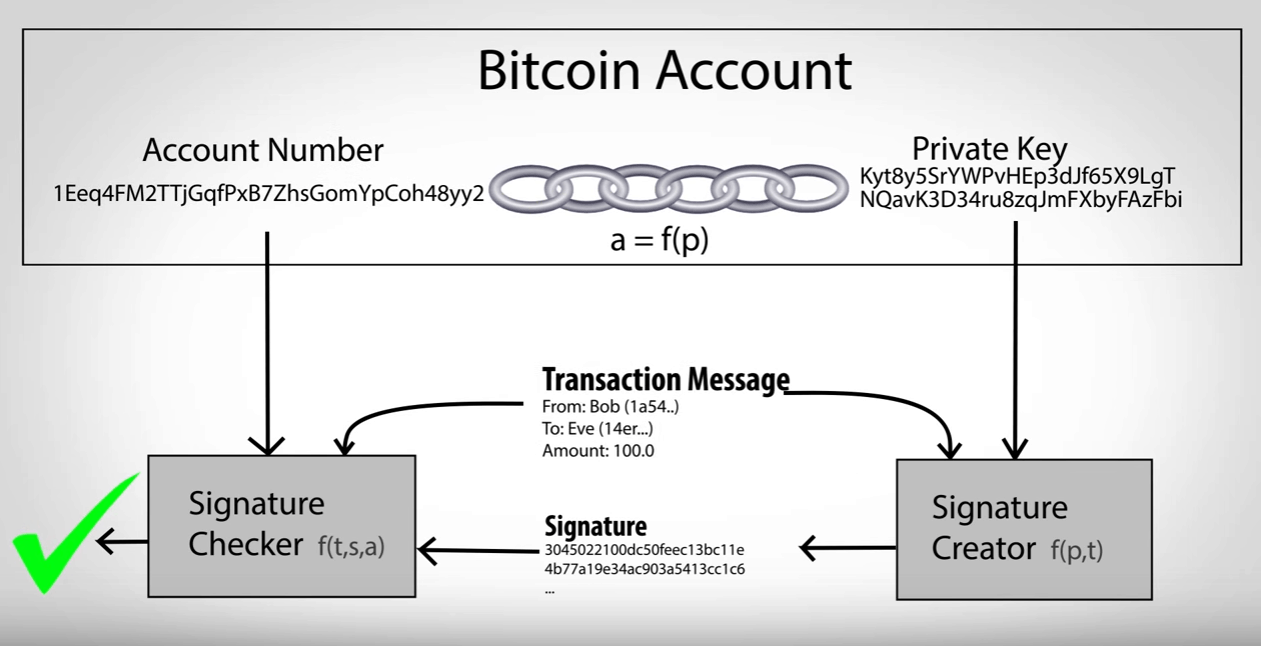
\includegraphics[width=11cm, height=7cm]{privatekey}
\end{frame}

\begin{frame}
  \frametitle{Hash Function}
  \begin{itemize}
    \item A hash function serves to fingerprint large data into a number.
    \item It is assumed that two different files will always have different hashes (injectivity)
   since the probability of two different files having the same hash is negligible.
    \item By the pigeon hole principle, the injectivity of the hash is impossible.
      However, two files that have the same hash were never found in SHA-256.
    \item It is also not possible to compute the inverse of the hash function.
  \end{itemize}
\end{frame}

\begin{frame}
  \frametitle{Cryptographic Functions}
  \begin{itemize}
    \item In Bitcoin, there is a private and a public key.
    \item From the private key, it is possible to generate a public key
 and to sign a transaction.
    \item It is not possible to know the private key from the public key and signature generated by it.
    \item It is possible to know if a signature and a public key coincide with the same private key that generates both of them.
    \item These functions are based on the SHA-256 hash function.
  \end{itemize}
\end{frame}

\begin{frame}
  \frametitle{Messages}
\begin{code}

variable
  MsgPrimitive : Set

data Msg : Set₁ where
  msgPrimitive : MsgPrimitive → Msg
  _+msg_ : Msg → Msg → Msg

infixr 5 _+msg_

record HasMsg (A : Set) : Set₁ where
  field
    toMsgPrimitive : A → MsgPrimitive
    invertMsg      : MsgPrimitive → A
    invertibleMsg  : ∀ x → invertMsg {A} (toMsgPrimitive x) ≡ x

open HasMsg
\end{code}

\AgdaHide{
\begin{code}
toMsg : {A : Set} ⦃ _ : HasMsg A ⦄ → A → Msg
toMsg {A} ⦃ record { toMsgPrimitive = toMsgPrimitive } ⦄ x
  = msgPrimitive {A} (toMsgPrimitive x)
\end{code}
}

\end{frame}

\begin{frame}
  \frametitle{Crypto Constants}
\begin{code}

module Crypto
  ⦃ _ : HasMsg ℕ ⦄
  (PublicKey : Set)
  (PrivateKey : Set)
  (Address : Set)
  ⦃ _ : HasMsg Address ⦄
  (Signature : Set)
  (Hashed : Set)
  where

  Amount = ℕ
  Time = ℕ
  BlockPosition = ℕ
\end{code}
\end{frame}

\begin{frame}
  \frametitle{Crypto Postulates}
\begin{code}

  record CryptoPostulates : Set₁ where
    field
      _priv≡pub_        : PrivateKey → PublicKey → Set
      publicKey2Address : PublicKey → Address
      Signed            : Msg → PublicKey → Signature → Set
      Signed?           : (msg : Msg) (pk : PublicKey)
        (sig : Signature) → Dec $ Signed msg pk sig
      hashMsg : Msg → Hashed
      hash-inj : ∀ m n
        → hashMsg m ≡ hashMsg n
        →         m ≡ n

  module CryptoWithPostulates
    (crypto-postulates : CryptoPostulates)
    where
\end{code}
\AgdaHide{
\begin{code}
    open CryptoPostulates crypto-postulates
\end{code}
}
\end{frame}

\begin{frame}
  \frametitle{Postulates}
  \begin{itemize}
    \item Hash injective is impossible to proof.
      But we postulate it because the probability of hash collision is very low.
    \item In my master thesis, each function of crypto was postulated.
      However, it is better to put these functions as variables.
      Therefore, the code can be more general for every crypto function that has these properties.
  \end{itemize}
\end{frame}

\section{Transactions}

\begin{frame}
  \frametitle{Message Signed}
\begin{code}
    record SignedWithSigPbk (msg : Msg)(address : Address)
      : Set where
      field
        publicKey   :  PublicKey
        pbkCorrect  :  publicKey2Address publicKey ≡ address
        signature   :  Signature
        signed      :  Signed msg publicKey signature

\end{code}
\end{frame}

\begin{frame}
   \frametitle{Transactions}
   \begin{itemize}
     \item With a transaction, it is possible to send Bitcoins from one account to another.
     \item Transactions are like a paper check. The individual specifies an amount and signs the transaction.
     \item In Bitcoin, there are two kinds of transactions:
       the coinbase transactions and the normal transaction.
       There is just one coinbase transaction per block and it has only outputs,
       while the normal transaction has inputs and outputs.
       The inputs of a transaction should be outputs of other transactions that have never been used as input of one transaction.
    \item Furthermore, each transaction must have a signature generated from the private key proving that the public key user agreed to make that transaction.
   \end{itemize}
\end{frame}

\begin{frame}
\begin{code}

    record TXField : Set where
      constructor txfield
      field
        amount  : Amount
        address : Address

    record TXFieldWithId : Set where
      constructor txfieldid
      field
        time     : Time
        position : ℕ
        txField  : TXField
      open TXField txField public
\end{code}
\end{frame}
% \begin{frame}
\AgdaHide{
\begin{code}
    removeId : TXFieldWithId → TXField
    removeId tx = txfield amount address
      where open TXFieldWithId tx

    data VectorOutput : (time : Time) (size : ℕ)
      (amount : Amount) → Set where
      fstEl : ∀ {time : Time}
        (tx : TXFieldWithId)
        (sameId : TXFieldWithId.time tx ≡ time)
        (elStart : TXFieldWithId.position tx ≡ zero)
        → VectorOutput time 1 (TXFieldWithId.amount tx)

      cons : ∀ {time : Time} {size : ℕ} {amount : Amount}
        (listOutput : VectorOutput time size amount)
        (tx : TXFieldWithId)
        (sameId : TXFieldWithId.time tx ≡ time)
        (elStart : TXFieldWithId.position tx ≡ size)
        → VectorOutput time (suc size)
          (amount + TXFieldWithId.amount tx)

-- \end{code}
-- \end{frame}
-- \begin{frame}
-- \begin{code}

    VectorOutput→List : ∀ {time : Time} {size : ℕ}
      {amount : Amount}
      (outs : VectorOutput time size amount)
      → List TXFieldWithId
    VectorOutput→List (fstEl tx sameId elStart) = tx ∷ []
    VectorOutput→List (cons outs tx sameId elStart) =
      tx ∷ VectorOutput→List outs

-- \end{code}
-- \end{frame}
-- \begin{frame}
-- \begin{code}

    TX→Msg : (tx : TXField) → Msg
    TX→Msg record { amount = amount ; address = address }
      = toMsg amount +msg toMsg address

    TXId→Msg : (tx : TXFieldWithId) → Msg
    TXId→Msg tx
      = toMsg time +msg toMsg position +msg
        toMsg amount +msg toMsg address
      where open TXFieldWithId tx

    txInput→Msg : (input : TXFieldWithId) (outputs : List TXField)
      → NonNil outputs → Msg
    txInput→Msg input [] ()
    txInput→Msg input (output ∷ []) _
      = TX→Msg output +msg TXId→Msg input
    txInput→Msg input (output ∷ out2 ∷ outputs) _
      = TX→Msg output +msg txInput→Msg input
        (out2 ∷ outputs) tt

    txEls→Msg : ∀ {inputs : List TXFieldWithId}
      (input : TXFieldWithId) (outputs : List TXFieldWithId)
      → NonNil inputs × NonNil outputs → Msg
    txEls→Msg input [] (_ , ())
    txEls→Msg input (output ∷ outputs) _
      = txInput→Msg input (map removeId (output ∷ outputs)) tt

-- \end{code}
-- \end{frame}
-- \begin{frame}
-- \begin{code}

    txEls→MsgVecOut :
      {time      : Time}
      {outSize   : ℕ}
      {outAmount : Amount}
      (input     : TXFieldWithId)
      (outputs   : VectorOutput time outSize outAmount)
      → Msg
    txEls→MsgVecOut input (fstEl tx sameId elStart)
      = TX→Msg (removeId tx) +msg TXId→Msg input
    txEls→MsgVecOut input (cons outputs tx sameId elStart) =
      TX→Msg (removeId tx) +msg
      txEls→MsgVecOut input outputs

    txFieldList→TotalAmount : (txs : List TXFieldWithId) → Amount
    txFieldList→TotalAmount [] = zero
    txFieldList→TotalAmount (x ∷ txs)
      = txFieldList→TotalAmount txs + TXFieldWithId.amount x
      where open TXFieldWithId

    record TXSigned
      {time} {outSize} {outAmount}
      (inputs    : List TXFieldWithId)
      (outputs   : VectorOutput time outSize outAmount)
        : Set where
      constructor txsig
      field
        nonEmpty : NonNil inputs
        signed   : All[ input ∈ inputs ]
          (SignedWithSigPbk (txEls→MsgVecOut input outputs)
          (TXFieldWithId.address input))
        in≥out : txFieldList→TotalAmount inputs ≥ outAmount

    NonEmptyList = λ A → Σ[ xs ∈ List A ] NonNil xs

    SignedWithSigPbk' : ∀
      {time} {outSize} {outAmount}
      (input    : TXFieldWithId)
      (outputs   : VectorOutput time outSize outAmount)
      → Set
    SignedWithSigPbk' input outputs = SignedWithSigPbk
      (txEls→MsgVecOut input outputs) (TXFieldWithId.address input)

    All' : {A : Set} (P : A → Set) → NonEmptyList A → Set
    All' P (x ∷ xs , tt) = All P (x ∷ xs)

    All'-syntax = All'
    syntax All'-syntax (λ x → P) xs = All'[ x ∈ xs ] P

    totalSpent : NonEmptyList TXFieldWithId → Amount
    totalSpent (x ∷ xs , tt) = txFieldList→TotalAmount (x ∷ xs)
\end{code}
}
% \end{frame}
\begin{frame}
\begin{code}

    record TXSigned'
      {time} {outSize} {outAmount}
      (inputs    : NonEmptyList TXFieldWithId)
      (outputs   : VectorOutput time outSize outAmount)
        : Set where
      constructor txsig
      field
        signed   : All'[ input ∈ inputs ]
          (SignedWithSigPbk' input outputs)
        in≥out : totalSpent inputs ≥ outAmount

\end{code}
\end{frame}
% \begin{frame}
\AgdaHide{
\begin{code}

    record TXSignedRawOutput
      (inputs : List TXFieldWithId)
      (outputs : List TXFieldWithId) : Set where
      field
        nonEmpty : NonNil inputs × NonNil outputs
        signed   : All[ input ∈ inputs ]
          (SignedWithSigPbk (txEls→Msg input outputs nonEmpty)
                          (TXFieldWithId.address input))
        in≥out : txFieldList→TotalAmount inputs
                 ≥ txFieldList→TotalAmount outputs

    txSigInput : {inputs : List TXFieldWithId}
      {outputs : List TXFieldWithId}
      (tx : TXSignedRawOutput inputs outputs)
      → List TXFieldWithId
    txSigInput {inputs} _ = inputs

\end{code}
}
% \end{frame}

\section{Blockchain}

\begin{frame}
  \frametitle{Blockchain constants}
\begin{code}
    module WithConstants
      (totalQtSub1 : ℕ)
      (blockReward : BlockPosition → Amount)
      where

      totalQt : ℕ
      totalQt = suc totalQtSub1

      tQtTxs : Set
      tQtTxs = Fin $ totalQt
\end{code}
\end{frame}

\begin{frame}
   \frametitle{Unspent Transaction Model}
   \begin{itemize}
     \item In the unspent transaction model, every transaction is added to the transaction tree.
     \item To find out the balance of an account it is necessary to look at all unspent transactions
       sent to that account.
     \item To transact the currency, it is necessary to use as input the outputs of
       other unspent transactions.
   \end{itemize}
\end{frame}

\begin{frame}
  \frametitle{Bitcoin UTXO}
    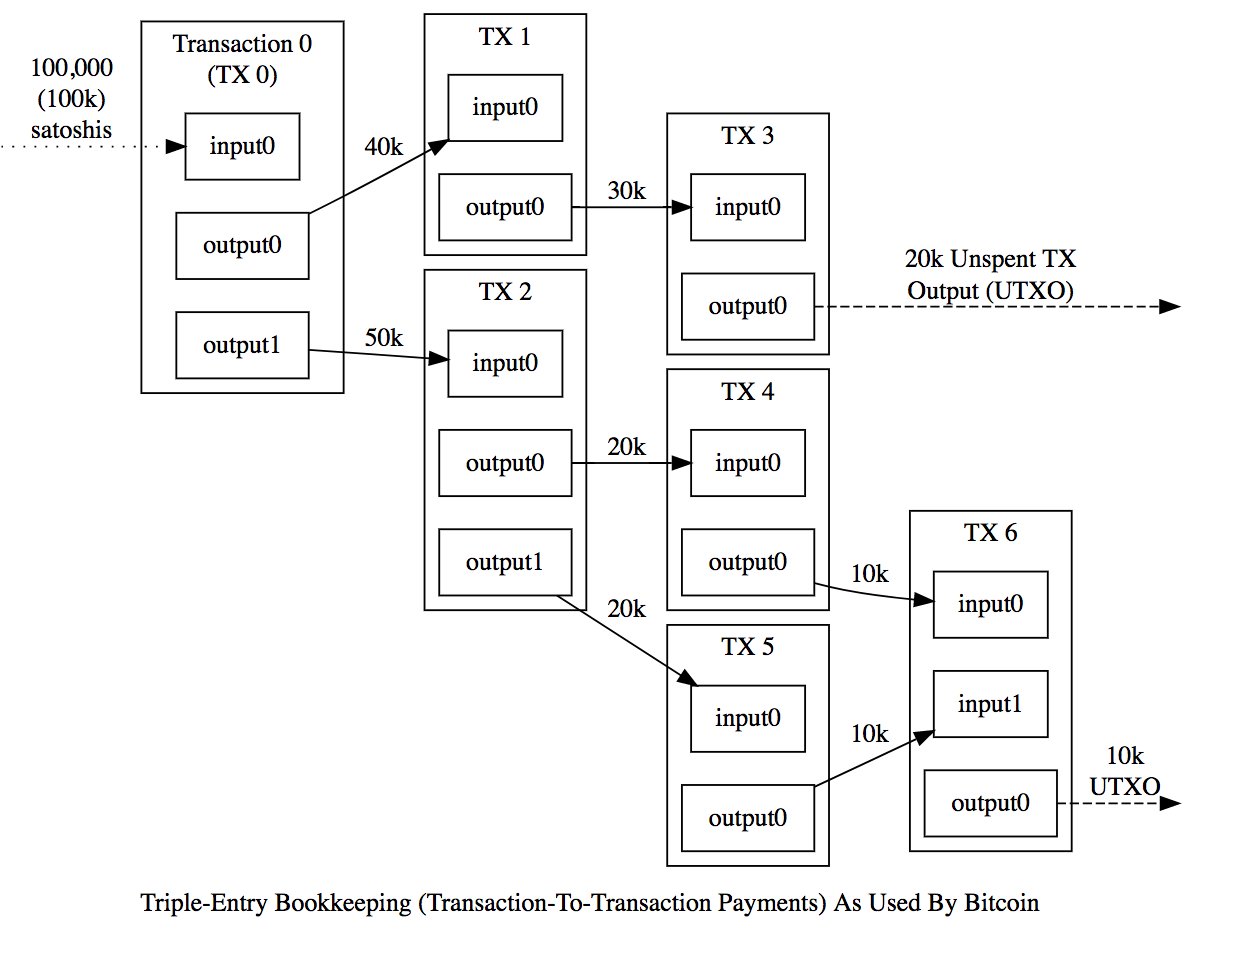
\includegraphics[width=11cm, height=7cm]{utxo}
\end{frame}

\begin{frame}
   \frametitle{Transaction Trees}
   \begin{itemize}
     \item The idea of the transaction tree is to gather all transactions into a tree.
     \item In this way, it is possible to fingerprint the information of all transactions calculating just their hash.
     \item With the injectivity property of the hash, it is possible to verify that two trees are equal in constant time complexity.
   \end{itemize}
\end{frame}

\begin{frame}
  \frametitle{Transaction tree}
    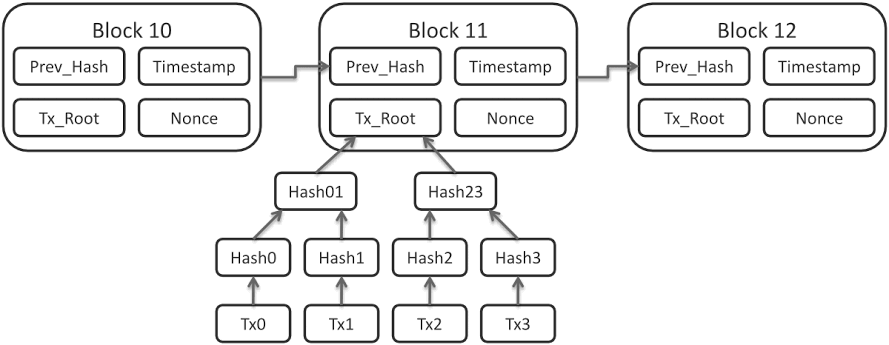
\includegraphics[width=10cm, height=5cm]{blockchain}
\end{frame}

% \begin{frame}
%   \frametitle{Transaction tree}
\AgdaHide{
\begin{code}

      mutual
        data TXTree : (time : Time) (block : BlockPosition)
          (outputs : List TXFieldWithId)
          (totalFees : Amount)
          (qtTransactions : tQtTxs) → Set where

          genesisTree : TXTree zero zero [] zero zero

\end{code}
}
% \end{frame}
% \begin{frame}
\AgdaHide{
\begin{code}

          txtree      :
            {block : BlockPosition} {time : Time}
            {outSize : ℕ} {amount : Amount}
            {inputs : List TXFieldWithId}
            {outputTX : VectorOutput time outSize amount}
            {totalFees : Amount} {qtTransactions : tQtTxs}
            (tree : TXTree time block inputs totalFees qtTransactions)
            (tx : TX {time} {block} {inputs} {outSize} tree outputTX)
            (proofLessQtTX :
                toℕ qtTransactions ≤ totalQtSub1
                ⊎
                (isCoinbase tx))
            → TXTree (suc time)
              (nextBlock tx)
              (inputsTX tx ++ VectorOutput→List outputTX)
              (incFees tx) (incQtTx tx proofLessQtTX)

\end{code}
}
% \end{frame}
% \begin{frame}
%   \frametitle{Transaction}
\AgdaHide{
\begin{code}

        data TX {time : Time} {block : BlockPosition}
            {inputs : List TXFieldWithId} {outSize : ℕ}
            {outAmount : Amount} {totalFees : ℕ}
            {qtTransactions : tQtTxs}
          : (tr : TXTree time block inputs totalFees qtTransactions)
            (outputs : VectorOutput time outSize outAmount)
            → Set where
          normalTX :
            (tr : TXTree time block inputs totalFees qtTransactions)
            (SubInputs : SubList inputs)
            (outputs : VectorOutput time outSize outAmount)
            (txSigned : TXSigned (sub→list SubInputs) outputs)
            → TX tr outputs

\end{code}
}
% \end{frame}
% \begin{frame}
\AgdaHide{
\begin{code}

          coinbase :
            (tr : TXTree time block inputs totalFees qtTransactions)
            (outputs : VectorOutput time outSize outAmount)
            (pAmountFee : outAmount out≡Fee totalFees
              +RewardBlock block)
            → TX tr outputs

\end{code}
}
% \end{frame}
% \begin{frame}
\AgdaHide{
\begin{code}

        isCoinbase : ∀ {block : BlockPosition} {time : Time}
          {inputs : List TXFieldWithId}
          {outSize : ℕ} {amount : Amount}
          {totalFees : ℕ} {qtTransactions : tQtTxs}
          {tr : TXTree time block inputs totalFees qtTransactions}
          {outputs : VectorOutput time outSize amount}
          (tx : TX {time} {block} {inputs} {outSize} tr outputs)
          → Set
        isCoinbase (normalTX _ _ _ _) = ⊥
        isCoinbase (coinbase _ _ _)     = ⊤

        nextBlock : ∀ {block : BlockPosition} {time : Time}
          {inputs : List TXFieldWithId}
          {outSize : ℕ} {amount : Amount}
          {totalFees : ℕ} {qtTransactions : tQtTxs}
          {tr : TXTree time block inputs totalFees qtTransactions}
          {outputs : VectorOutput time outSize amount}
          (tx : TX {time} {block} {inputs} {outSize} tr outputs)
          → ℕ

-- \end{code}
-- \end{frame}
-- \begin{frame}
-- \begin{code}

        nextBlock (normalTX genesisTree _ _ _) = zero
        nextBlock {block} (normalTX (txtree _
          (normalTX _ _ _ _) _) _ _ _) = block
        nextBlock {block} (normalTX (txtree _
          (coinbase _ _ _) _) _ _ _) = suc block
        nextBlock (coinbase genesisTree _ _) = zero
        nextBlock {block} (coinbase (txtree _
          (normalTX _ _ _ _) _) _ _) = block
        nextBlock {block} (coinbase (txtree _
          (coinbase _ _ _) _) _ _) = suc block

-- \end{code}
-- \end{frame}
-- \begin{frame}
-- \begin{code}

        inputsTX : ∀ {block : BlockPosition} {time : Time}
          {inputs : List TXFieldWithId}
          {outSize : ℕ} {amount : Amount}
          {totalFees : ℕ} {qtTransactions : tQtTxs}
          {tr : TXTree time block inputs totalFees qtTransactions}
          {outputs : VectorOutput time outSize amount}
          (tx : TX {time} {block} {inputs} {outSize} tr outputs)
          → List TXFieldWithId
        inputsTX (normalTX _ SubInputs _ _) = list-sub SubInputs
        inputsTX {_} {_} {inputs} (coinbase _ _ _) = inputs

-- \end{code}
-- \end{frame}
-- \begin{frame}
-- \begin{code}

        postulate
          incQtTx : ∀ {qtTransactions : tQtTxs}
            {block : BlockPosition} {time : Time}
            {inputs : List TXFieldWithId}
            {outSize : ℕ} {amount : Amount}
            {totalFees : ℕ}
            {tr : TXTree time block inputs totalFees qtTransactions}
            {outputs : VectorOutput time outSize amount}
            (tx : TX {time} {block} {inputs} {outSize} tr outputs)
            (proofLessQtTX :
                toℕ qtTransactions ≤ totalQtSub1
                ⊎
                (isCoinbase tx))
            → tQtTxs

-- \end{code}
-- \end{frame}
-- \begin{frame}
-- \begin{code}

        incFees : ∀ {block : BlockPosition} {time : Time}
          {inputs : List TXFieldWithId}
          {outSize : ℕ} {amount : Amount}
          {totalFees : Amount} {qtTransactions : tQtTxs}
          {tr : TXTree time block inputs totalFees qtTransactions}
          {outputs : VectorOutput time outSize amount}
          (tx : TX {time} {block} {inputs} {outSize} tr outputs)
          → Amount
        incFees {_} {_} {_} {_} {amount} {totalFees}
          (normalTX _ SubInputs _ (txsig _ _ in≥out)) =
          txFieldList→TotalAmount (sub→list SubInputs)
          - amount p≥ in≥out
          + totalFees
        incFees (coinbase tr outputs _) = zero

-- \end{code}
-- \end{frame}
-- \begin{frame}
-- \begin{code}

        _out≡Fee_+RewardBlock_ : (amount : Amount)
          (totalFees : Amount)
          (block : BlockPosition) → Set
        amount out≡Fee totalFees +RewardBlock block =
          amount ≡ totalFees + blockReward block

-- \end{code}
-- \end{frame}
-- \begin{frame}
-- \begin{code}


      data nextTXTree :
        {block₁ : BlockPosition}
        {time₁ : Time}
        {outputs₁ : List TXFieldWithId}
        {totalFees₁ : Amount}
        {qtTransactions₁ : tQtTxs}
        (txTree₁ : TXTree time₁ block₁ outputs₁
          totalFees₁ qtTransactions₁)

        {block₂ : BlockPosition}
        {time₂ : Time}
        {outputs₂ : List TXFieldWithId}
        {totalFees₂ : Amount}
        {qtTransactions₂ : tQtTxs}
        (txTree₂ : TXTree time₂ block₂ outputs₂
          totalFees₂ qtTransactions₂)
        → Set where

-- \end{code}
-- \end{frame}
-- \begin{frame}
-- \begin{code}

        firstTX : ∀ {block time outputs totalFees qtTransactions}
          (txTree : TXTree time block outputs totalFees qtTransactions)
          → nextTXTree txTree txTree
        nextTX : ∀ {block₁ time₁ outputs₁ totalFees₁ qtTransactions₁}
          {txTree₁ : TXTree time₁ block₁
            outputs₁ totalFees₁ qtTransactions₁}

          {block₂ time₂ outputs₂ totalFees₂ qtTransactions₂}
          {txTree₂ : TXTree time₂ block₂
            outputs₂ totalFees₂ qtTransactions₂}

          (nxTree : nextTXTree txTree₁ txTree₂)

-- \end{code}
-- \end{frame}
-- \begin{frame}
-- \begin{code}

          {outSize amount}
          {outputTX : VectorOutput time₂ outSize amount}
          (tx : TX txTree₂ outputTX)
          (proofLessQtTX :
              toℕ qtTransactions₂ ≤ totalQtSub1
              ⊎
              (isCoinbase tx))
          → nextTXTree txTree₁ (txtree txTree₂ tx proofLessQtTX)

-- \end{code}
-- \end{frame}
-- \begin{frame}
-- \begin{code}

      firstTreesInBlock : ∀
        {block time outputs totalFees qtTransactions}
        (tree : TXTree time block outputs totalFees qtTransactions)
        → Set
      firstTreesInBlock genesisTree = ⊤
      firstTreesInBlock (txtree genesisTree _ _) = ⊥
      firstTreesInBlock (txtree (txtree _
        (normalTX _ _ _ _) _) _ _) = ⊥
      firstTreesInBlock (txtree (txtree _
        (coinbase _ _ _) _) _ _) = ⊤

-- \end{code}
-- \end{frame}
-- \begin{frame}
-- \begin{code}

      isFirstTreeInBlock : ∀
        {block time outputs totalFees qtTransactions}
        (tree : TXTree time block outputs totalFees qtTransactions)
        → Dec (firstTreesInBlock tree)
      isFirstTreeInBlock genesisTree = yes tt
      isFirstTreeInBlock (txtree genesisTree
        (normalTX _ _ _ _) _) = no λ x → x
      isFirstTreeInBlock (txtree genesisTree
        (coinbase _ _ _) _) = no λ x → x
      isFirstTreeInBlock (txtree (txtree _
        (normalTX _ _ _ _) _) _ _) = no λ x → x
      isFirstTreeInBlock (txtree (txtree _
        (coinbase _ _ _) _) _ _) = yes tt

-- \end{code}
-- \end{frame}
-- \begin{frame}
-- \begin{code}

      coinbaseTree : ∀
        {block time outputs totalFees qtTransactions}
        (tree : TXTree time block outputs totalFees qtTransactions)
        → Set
      coinbaseTree genesisTree = ⊥
      coinbaseTree (txtree _ (normalTX _ _ _ _) _) = ⊥
      coinbaseTree (txtree _ (coinbase _ _ _) _) = ⊤

\end{code}
}
% \end{frame}

\begin{frame}
   \frametitle{Blocks and Blockchain}
   \begin{itemize}
     \item Transactions are embedded in blocks where they are stored.
     \item In Bitcoin, there is a chain of blocks: the blockchain.
       The first block is called the genesis block and every 10 minutes, on average, a new block is added to this blockchain.
     \item There is a limit of transactions that each block can have (in Bitcoin, it is 10 MB of data).
       Therefore, it is important to pay a transaction fee for it to be included in the blockchain.
     \item If there are two blockchains on different computers, it is considered the valid blockchain the one with the most blocks.
   \end{itemize}
\end{frame}

\begin{frame}
\frametitle{Blockchain}
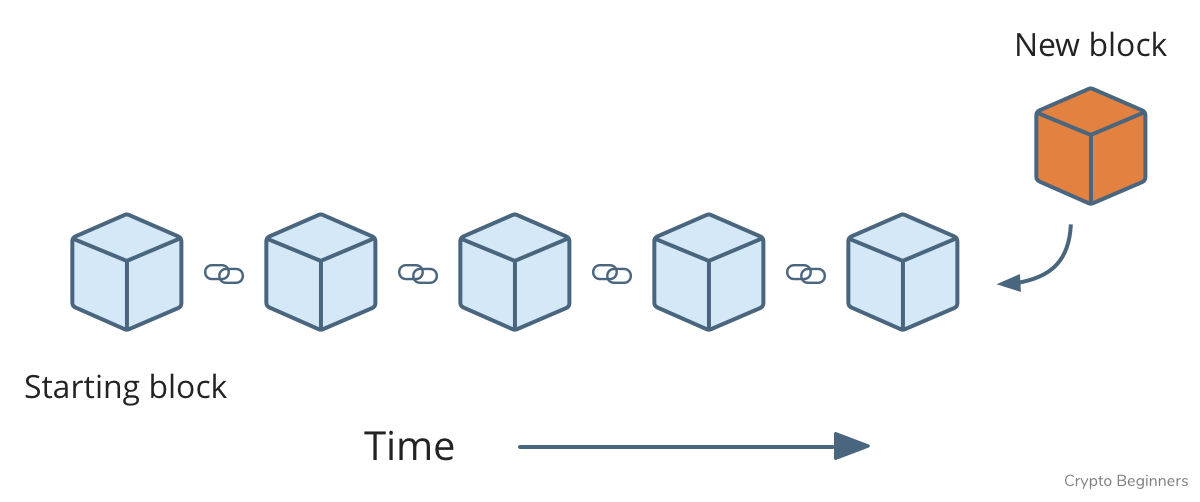
\includegraphics[width=11cm, height=8cm]{blockchain1}
\end{frame}

\begin{frame}
\frametitle{Blockchain}
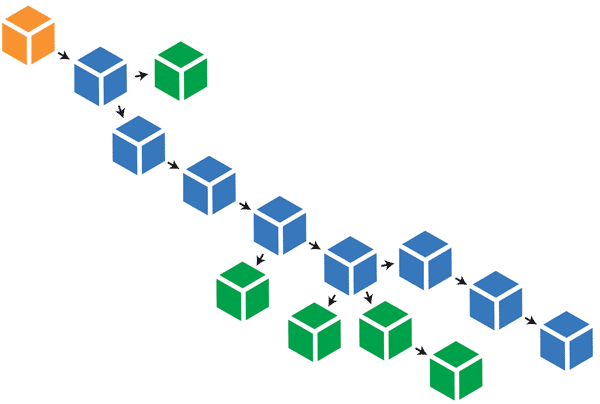
\includegraphics[width=11cm, height=8cm]{blockchain2}
\end{frame}

% \begin{frame}
%   \frametitle{Block}
\AgdaHide{
\begin{code}

      record Block
        {block₁ : BlockPosition}
        {time₁ : Time}
        {outputs₁ : List TXFieldWithId}
        {totalFees₁ : Amount}
        {qtTransactions₁ : tQtTxs}
        (txTree₁ : TXTree time₁ block₁ outputs₁
          totalFees₁ qtTransactions₁)

        {time₂ : Time}
        {outputs₂ : List TXFieldWithId}
        {totalFees₂ : Amount}
        {qtTransactions₂ : tQtTxs}
        (txTree₂ : TXTree time₂ block₁ outputs₂
          totalFees₂ qtTransactions₂)
        : Set where

\end{code}
}
% \end{frame}
% \begin{frame}
%   \frametitle{Block}
\AgdaHide{
\begin{code}

        constructor blockc
        field
          nxTree           : nextTXTree txTree₁ txTree₂
          fstBlock         : firstTreesInBlock txTree₁
          sndBlockCoinbase : coinbaseTree txTree₂

\end{code}
}
% \end{frame}
% \begin{frame}
\AgdaHide{
\begin{code}

      fstTree→coinbase : ∀
        {block time outputs totalFees qtTransactions}
        {tree : TXTree time block outputs totalFees qtTransactions}
        {outSize amount}
        {outputTX : VectorOutput time outSize amount}
        {tx : TX tree outputTX}
        {proofLessQtTX :
            toℕ qtTransactions ≤ totalQtSub1
            ⊎
            (isCoinbase tx)}
        (fstTree : firstTreesInBlock (txtree tree tx proofLessQtTX))
        → coinbaseTree tree

-- \end{code}
-- \end{frame}
-- \begin{frame}
-- \begin{code}

      fstTree→coinbase {_} {_} {_} {_} {_} {genesisTree} ()
      fstTree→coinbase {_} {_} {_} {_} {_}
        {txtree _ (normalTX _ _ _ _) _} ()
      fstTree→coinbase {_} {_} {_} {_} {_}
        {txtree _ (coinbase _ _ _) _} _ = tt

\end{code}
}
% \end{frame}
% \begin{frame}
%   \frametitle{Blockchain}
\AgdaHide{
\begin{code}

      data Blockchain :
        {block₁ : BlockPosition}
        {time₁ : Time}
        {outputs₁ : List TXFieldWithId}
        {totalFees₁ : Amount}
        {qtTransactions₁ : tQtTxs}
        {txTree₁ : TXTree time₁ block₁ outputs₁
          totalFees₁ qtTransactions₁}

        {time₂ : Time}
        {outputs₂ : List TXFieldWithId}
        {totalFees₂ : Amount}
        {qtTransactions₂ : tQtTxs}
        {txTree₂ : TXTree time₂ block₁ outputs₂ totalFees₂
          qtTransactions₂}
        (block : Block txTree₁ txTree₂)
        → Set where

\end{code}
}
% \end{frame}
% \begin{frame}
%   \frametitle{Blockchain}
\AgdaHide{
\begin{code}

          fstBlock' :
            {block₁ : BlockPosition}
            {time₁ : Time}
            {outputs₁ : List TXFieldWithId}
            {totalFees₁ : Amount}
            {qtTransactions₁ : tQtTxs}
            {txTree₁ : TXTree time₁ block₁ outputs₁ totalFees₁
              qtTransactions₁}

            {time₂ : Time}
            {outputs₂ : List TXFieldWithId}
            {totalFees₂ : Amount}
            {qtTransactions₂ : tQtTxs}
            {txTree₂ : TXTree time₂ block₁ outputs₂ totalFees₂
              qtTransactions₂}
            (block : Block txTree₁ txTree₂)
            → Blockchain block

\end{code}
}
% \end{frame}
% \begin{frame}
%   \frametitle{Blockchain}
\AgdaHide{
\begin{code}

          addBlock :
            {block-p₁ : ℕ}
            {time-p₁ : Time}
            {outputs-p₁ : List TXFieldWithId}
            {totalFees-p₁ : Amount}
            {qtTransactions-p₁ : tQtTxs}
            {txTree-p₁ : TXTree time-p₁ block-p₁
              outputs-p₁ totalFees-p₁ qtTransactions-p₁}

            {time-p₂ : Time}
            {outputs-p₂ : List TXFieldWithId}
            {totalFees-p₂ : Amount}
            {qtTransactions-p₂ : tQtTxs}
            {txTree-p₂ : TXTree time-p₂ block-p₁
              outputs-p₂ totalFees-p₂ qtTransactions-p₂}
            {block-p : Block txTree-p₁ txTree-p₂}
            (blockchain : Blockchain block-p)

\end{code}
}
% \end{frame}
% \begin{frame}
%   \frametitle{Blockchain}
\AgdaHide{
\begin{code}

            {outSize : ℕ}
            {amount : Amount}
            {outputTX : VectorOutput time-p₂ outSize amount}
            {tx : TX {time-p₂} {block-p₁}
              {outputs-p₂} {outSize} txTree-p₂ outputTX}
            {proofLessQtTX :
                toℕ qtTransactions-p₂ ≤ totalQtSub1
                ⊎
                (isCoinbase tx)}

            {time₂ : Time}
            {outputs₂ : List TXFieldWithId}
            {totalFees₂ : Amount}
            {qtTransactions₂ : tQtTxs}
            {txTree₂ : TXTree time₂ (nextBlock tx) outputs₂
              totalFees₂ qtTransactions₂}
            (block : Block (txtree txTree-p₂ tx proofLessQtTX)
              txTree₂)
            → Blockchain block

\end{code}
}
% \end{frame}
% \begin{frame}
\AgdaHide{
\begin{code}

      record RawBlock
        {block : BlockPosition}
        {time₂ : Time}
        {outputs₂ : List TXFieldWithId}
        {totalFees₂ : Amount}
        {qtTransactions₂ : tQtTxs}
        (tree₂ : TXTree time₂ block outputs₂ totalFees₂
          qtTransactions₂)
        : Set where
        constructor rawBlockc

-- \end{code}
-- \end{frame}
-- \begin{frame}
-- \begin{code}

        field
          {time}           : Time
          {outputs}        : List TXFieldWithId
          {totalFees}      : Amount
          {qtTransactions} : tQtTxs
          {tree}           : TXTree time block
            outputs totalFees qtTransactions
          rawBlock         : Block tree tree₂

-- \end{code}
-- \end{frame}
-- \begin{frame}
-- \begin{code}

      isCoinbaseTree : ∀
        {block time outputs totalFees qtTransactions}
        (tree : TXTree time block outputs totalFees qtTransactions)
        → Dec (coinbaseTree tree)
      isCoinbaseTree genesisTree = no λ x → x
      isCoinbaseTree (txtree _ (normalTX _ _ _ _) _) = no λ x → x
      isCoinbaseTree (txtree _ (coinbase _ _ _) _) = yes tt

-- \end{code}
-- \end{frame}
-- \begin{frame}
-- \begin{code}

      record fstTree
        {block : BlockPosition}
        {time₂ : Time}
        {outputs₂ : List TXFieldWithId}
        {totalFees₂ : Amount}
        {qtTransactions₂ : tQtTxs}
        (txTree₂ : TXTree time₂ block outputs₂
          totalFees₂ qtTransactions₂)
        : Set where
        constructor fstTreec

-- \end{code}
-- \end{frame}
-- \begin{frame}
-- \begin{code}

        field
          {time}               : Time
          {outputs}            : List TXFieldWithId
          {totalFees}          : Amount
          {qtTransactions}     : tQtTxs
          {tree}               : TXTree time block
            outputs totalFees qtTransactions
          nxTree               : nextTXTree tree txTree₂
          fstBlockc            : firstTreesInBlock tree

-- \end{code}
-- \end{frame}
-- \begin{frame}
-- \begin{code}

      record fstTree₂
        {block : BlockPosition}
        {time₂ : Time}
        {outputs₂ : List TXFieldWithId}
        {totalFees₂ : Amount}
        {qtTransactions₂ : tQtTxs}
        (txTree₂ : TXTree time₂ block outputs₂ totalFees₂
          qtTransactions₂)
        : Set where
        pattern
        constructor fstTreec₂

-- \end{code}
-- \end{frame}
-- \begin{frame}
-- \begin{code}

        field
          {block₂}              : ℕ
          {time}               : Time
          {outputs}            : List TXFieldWithId
          {totalFees}          : Amount
          {qtTransactions}     : tQtTxs
          {tree}               : TXTree time block₂
            outputs totalFees qtTransactions
          eq                   : block ≡ block₂
          nxTree               : nextTXTree tree txTree₂
          fstBlockc            : firstTreesInBlock tree

-- \end{code}
-- \end{frame}
-- \begin{frame}
-- \begin{code}

      fstTree₂→fstTree : ∀
        {block time₂ outputs₂ totalFees₂ qtTransactions₂}
        {txTree₂ : TXTree time₂ block outputs₂ totalFees₂
          qtTransactions₂}
        (fTree₂ : fstTree₂ txTree₂)
        → fstTree txTree₂
      fstTree₂→fstTree (fstTreec₂ refl nxTree fstBlockc)
        = fstTreec nxTree fstBlockc

-- \end{code}
-- \end{frame}
-- \begin{frame}
-- \begin{code}

      record fstTreeChange
        (block : BlockPosition)
        (time : Time)
        (outputs : List TXFieldWithId)
        (totalFees : Amount)
        (qtTransactions : tQtTxs)
        : Set where
        constructor fstTreeChangedc
        field
          {tree}      : TXTree time block outputs
            totalFees qtTransactions
          ftree       : fstTree tree

-- \end{code}
-- \end{frame}
-- \begin{frame}
-- \begin{code}

      changeBlockType : ∀
        {block block₂ time outputs totalFees qtTransactions}
        {tree : TXTree time block outputs totalFees qtTransactions}
        {txTree : TXTree time block outputs
          totalFees qtTransactions}
        (fstTree : fstTree tree)
        (eq : block ≡ block₂)
        → fstTreeChange block₂ time outputs
          totalFees qtTransactions
      changeBlockType fstTree refl = fstTreeChangedc fstTree

-- \end{code}
-- \end{frame}
-- \begin{frame}
-- \begin{code}

      record TXChange
        {block : ℕ}
        {outSize : ℕ}
        {amount : ℕ}
        {time : Time}
        {block : BlockPosition}
        {outputs : List TXFieldWithId}
        {outputTX : VectorOutput time outSize amount}
        {totalFees : Amount}
        {qtTransactions : tQtTxs}
        (tree : TXTree time block outputs totalFees qtTransactions)
        (tx : TX tree outputTX)

-- \end{code}
-- \end{frame}
-- \begin{frame}
-- \begin{code}

        (proofLess :
          toℕ qtTransactions ≤ totalQtSub1
          ⊎
          (isCoinbase tx))
        : Set where
        constructor TXChangedc
        field
          fTree                 : fstTree (txtree tree tx proofLess)

-- \end{code}
-- \end{frame}
-- \begin{frame}
-- \begin{code}


      changeTXType : ∀
        {block time₁ time₂ totalFees₁ totalFees₂
          outputs₁ outputs₂ qtTransactions₁ qtTransactions₂
        outSize amount}
        {outputTX : VectorOutput time₂ outSize amount}
        {tree : TXTree time₁ block
          outputs₁ totalFees₁ qtTransactions₁}
        {tree₂ : TXTree time₂ block outputs₂
          totalFees₂ qtTransactions₂}
        (nxTree : nextTXTree tree tree₂)
        (fstBlockc : firstTreesInBlock tree)
        (tx : TX tree₂ outputTX)

-- \end{code}
-- \end{frame}
-- \begin{frame}
-- \begin{code}

        (proofLess :
          toℕ qtTransactions₂ ≤ totalQtSub1
          ⊎
          (isCoinbase tx))
        (eq : nextBlock tx ≡ block)
        → TXChange {block} tree₂ tx proofLess
      changeTXType nxTree fblock tx proof eq =
        let nxTX = nextTX nxTree tx proof
            ftree = fstTree₂→fstTree (fstTreec₂ eq nxTX fblock)
        in TXChangedc ftree

-- \end{code}
-- \end{frame}
-- \begin{frame}
-- \begin{code}


      fstTreeBlock : ∀
        {block time outputs totalFees qtTransactions}
        {tree : TXTree time block outputs totalFees qtTransactions}
        (fstTree : fstTree tree)
        → ℕ
      fstTreeBlock {block} _ = block

      firstTree : ∀
        {block time outputs totalFees qtTransactions}
        (tree : TXTree time block outputs totalFees qtTransactions)
        → fstTree tree
      firstTree genesisTree = fstTreec (firstTX genesisTree) tt

-- \end{code}
-- \end{frame}
-- \begin{frame}
-- \begin{code}

      firstTree {block₂} (txtree {block₁} tree tx proofLessQtTX)
        with isFirstTreeInBlock (txtree tree tx proofLessQtTX)
      ... | yes isFirst = fstTreec
        (firstTX (txtree tree tx proofLessQtTX)) isFirst
      ... | no ¬first with block₂ ≟ block₁
      ...   | yes eq = let ftree = firstTree tree
                           nxTree = fstTree.nxTree ftree
                           fstBlock = fstTree.fstBlockc ftree
                           chgType = changeTXType nxTree
                             fstBlock tx proofLessQtTX eq
                       in TXChange.fTree chgType
      ...   | no ¬eq = ⊥-elim impossible
                where postulate impossible : ⊥

-- \end{code}
-- \end{frame}
-- \begin{frame}
-- \begin{code}

      txTree→Block : ∀
        {block time outputs totalFees qtTransactions}
        (tree : TXTree time block outputs totalFees qtTransactions)
        → Dec (RawBlock tree)
      txTree→Block genesisTree =
        no λ { (rawBlockc (blockc _ _ sndBlockCoinbase))
        → sndBlockCoinbase }

-- \end{code}
-- \end{frame}
-- \begin{frame}
-- \begin{code}

      txTree→Block (txtree tree tx proofLessQtTX)
        with isCoinbaseTree (txtree tree tx proofLessQtTX)
      ... | no ¬isCoinbase =
              no λ{ (rawBlockc (blockc _ _ coinbaseTree))
                → ¬isCoinbase coinbaseTree}
      ... | yes isCoinbase = let fTree = firstTree
                                   (txtree tree tx proofLessQtTX)
                                 nxTree = fstTree.nxTree fTree
                                 fBlock = fstTree.fstBlockc fTree
                             in yes (rawBlockc
                               (blockc nxTree fBlock isCoinbase))

-- \end{code}
-- \end{frame}
-- \begin{frame}
-- \begin{code}

      {-# TERMINATING #-}
      block→blockchain : ∀
        {block₁ time₁ outputs₁ totalFees₁ qtTransactions₁}
        {txTree₁ : TXTree time₁ block₁ outputs₁
          totalFees₁ qtTransactions₁}
        {time₂ outputs₂ totalFees₂ qtTransactions₂}
        {txTree₂ : TXTree time₂ block₁ outputs₂
          totalFees₂ qtTransactions₂}
        (block : Block txTree₁ txTree₂)
        → Blockchain block
      block→blockchain {_} {_} {_} {_} {_} {genesisTree}
        (blockc nxTree fstBlock₁ sndBlockCoinbase) =
        fstBlock' (blockc nxTree tt sndBlockCoinbase)

-- \end{code}
-- \end{frame}
-- \begin{frame}
-- \begin{code}

      block→blockchain {_} {_} {_} {_} {_} {txtree tree tx
        proofLessQtTX}
        (blockc nxTree fstBlock₁ sndBlockCoinbase)
        with firstTree tree
      ... | fstTreec nxTree₁ fstBlockc = addBlock
        (block→blockchain (blockc nxTree₁ fstBlockc
          (fstTree→coinbase fstBlock₁)))
        (blockc nxTree fstBlock₁ sndBlockCoinbase)
\end{code}
}
% \end{frame}

\begin{frame}
   \frametitle{Mining}
   \begin{itemize}
     \item Every block has a cryptographic problem to be solved. That is,
       you need to calculate a nonce value such that the block hash is less than a specified value.
     \item This specified value is calculated from the average of the last 2016 blocks (2 weeks)
       so that the average block mining is 10 minutes.
   \end{itemize}
\end{frame}

\section{Conclusion}

\begin{frame}{Conclusions}
  \begin{itemize}
    \item In this work, all specifications were placed on types.
    \item In other works, the approach may be different.
      That is, without any information on types and all proofs done separately.
    \item This approach was not chosen as it is much simpler to understand the code when types are more expressive.
  \end{itemize}
\end{frame}

\begin{frame}{Missing Details}
  \begin{itemize}
    \item Calculate block hash and block nounce field.
    \item Change protocol to receive entire block instead of individual transactions.
    \item Add if there is a blockchain larger than the server's size.
  \end{itemize}
\end{frame}

\begin{frame}{More complex parts to add}
  \begin{itemize}
    \item Formal modeling of the blockchain as a distributed system.
    \item Create client code to interact with nodes.
    \item Specify the protocol between client and node and between node to node.
          However, adding the evidence to the raw data that the client sends has already been coded,
          which is the most complex part.
    \item Add a scripting language to the cryptocurrency.
  \end{itemize}
\end{frame}

\section{End}

\begin{frame}
  \vspace*{36 pt}
  \begin{center}
  {\Huge Questions?}
  \end{center}
\end{frame}

% \begin{frame}{Bibliographic references}
%   \bibliographystyle{apacite}
%   \bibliography{References}
% \end{frame}

\end{document}
